\chapter{Introduction}

% \section{Purpose}
% 
% Introduce core concepts relating to my project such as:

% \begin{enumerate}
% \item \chkBoxX Importance of Dengue and Malaria
% \item \chkBoxX Transmission cycle dependent on Mosquitoes
% \item \chkBox Limited effectiveness (medical/finacial) of treatment of the diseases in rural poor human communities
% \item \chkBoxX Vector Control Strategies
% \item \chkBoxX How Transgenesis modifies the vector control landscape
% \item \chkBox Elements of Successful Transgenesic Vector Control
% \item \chkBoxX Introduction to control of transcription and imoprtance of \glspl{CRE}/\glspl{CRM}
% \end{enumerate}




\section{Dengue fever and malaria are mosquito borne diseases}

There are many mosquito borne diseases that afflict the world's population.
Dengue fever and malaria are two important such diseases resulting in major health and productivity deficits in many developing nations worldwide \CITEME.
The causative agents of these two diseases are a suite of four species of RNA viruses (Dengue Virus 1-4) and a group of five species of protist from the genus \textit{Plasmodium} (\Plf, \Pv, \Po, \Pm, and \Pk).
However, in any \textbf{single} geographic location each disease is primarily transmitted by a single species of mosquito \CITEME (Table \ref{tab:species-disease-region}). 


\begin{table}[h]
\centering \sffamily
\begin{tabular}{lll}
\toprule
\textbf{Disease} & \textbf{Region} & \textbf{Mosquito Vector}\\ \midrule
Dengue Viruses & Wolrdwide & \Aea\\
\multirow{2}{*}{Human Malaria} & Africa & \Ang\\
 & Asia & \Ans\\\bottomrule
\end{tabular}

\caption[Primary geographic vectors of dengue fever and malaria]{\bsf{Primary geographic vectors of dengue fever and malaria}}\label{tab:species-disease-region}
\end{table} 


% +------------------+------------+-----------------------+
% | Disease          | Region     | Mosquito Vector       |
% +==================+============+=======================+
% | Dengue Viruses   | Worldwide  | *Aedes aeygypti*      |
% +------------------+------------+-----------------------+
% |                  | Africa     | *Anopheles gambiae*   |
% | Human Malaria    +------------+-----------------------+
% |                  | Asia       | *Anopheles stephensi* |
% +------------------+------------+-----------------------+

The fact that both of these diseases are caused by multiple pathogen species complicates efforts to prevent human disease: particularly when addressed from the perspective of providing therapeutic or prophylactic care directly to human patients.

\alert{TONY: MORE HERE ABOUT WHY THIS COMPLICATES THINGS?}

\section{Hematophagy (bloodfeeding) is an essential part of mosquito-borne disease}

Another very important aspect of both of these diseases is that people do not become infected through interaction with other people, and mosquitoes do not become infected through interaction with other mosquitoes.
The transmission cycles transmission of both diseases require that the pathogen be passed from human to mosquito or from mosquito to human.
This pattern has important consequences that can be exploited to reduce the number of people who will become infected with dengue fever or malaria.

\subsection{Transmission cycle}

\textbf{In Brief:}
\begin{enumerate}
\item A female mosquito bites an infected person.
\item The pathogen is taken into the mosquito's midgut along with bloodmeal.
\item The pathogen must escape the midgut and gain access to the mosquito's circulatory system (the animal is now \textbf{infected}).
\item The pathogen must gain access to the mosquito's salivary glands (the animal is now \textbf{infectious}).
\item The infectious female mosquito bites an uninfected human and the pathogens in her saliva are introduced to the person's body as she feeds.
\end{enumerate}


\begin{figure}[h]
\centering 
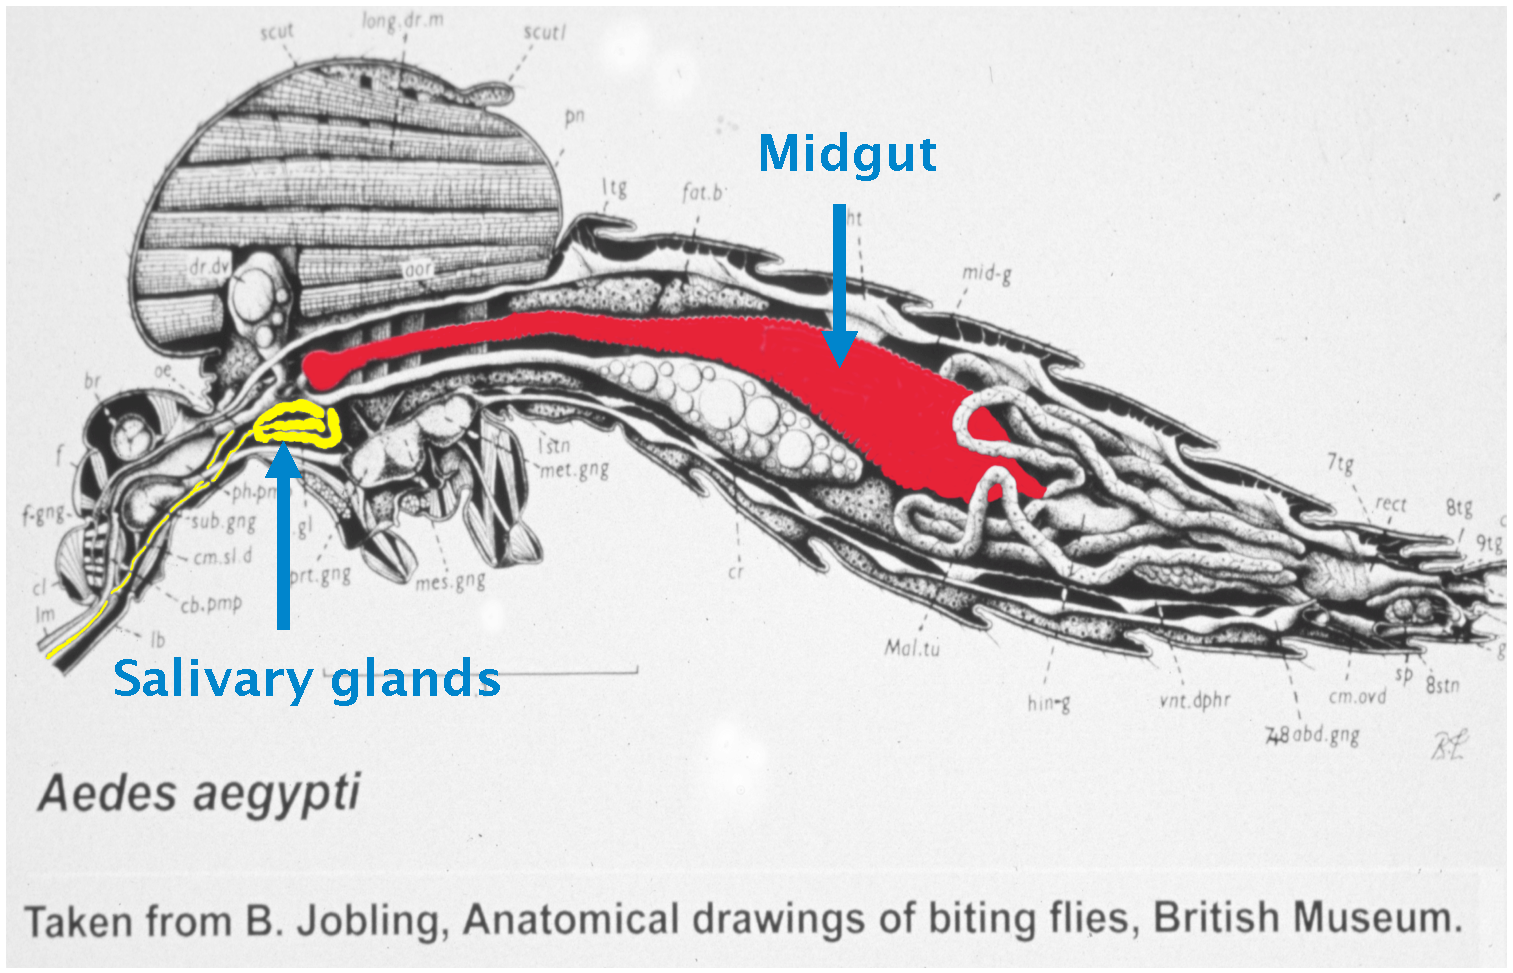
\includegraphics[width=.6\linewidth]{figures/figs/mosqXsection.pdf}
\caption[Cross section of a female mosquito]{\sf \textbf{Cross section of a female mosquito with tissues important to the transmission cycle highlighted.} \\  \cite{Jobling1987}}\label{fig:mosq-xsection}
\end{figure}


While the specifics of how viruses and protists live and reproduce in mosquitoes and humans are quite different, the transmission cycles of dengue and malaria are very similar in their critical events.
The transmission cycle of either pathogen type can be encapsulated into five fundamental events.
First, a female mosquito feeds on an infected human's blood taking up the pathogen as well (Figure \ref{fig:mosq-xsection}).
The bloodmeal is digested in the mosquito's midgut, and escape from the midgut is the first crucial step for the survival of the pathogen inside the mosquito.
If it is trapped in the midgut, it will eventually be passed as waste after the bloodmeal is digested.
If it manages to escape to the \gls{hemolymph}, the pathogen must survive long enough to gain access to the mosquito's salivary glands.
If it is unable to infiltrate the salivary glands, then the mosquito, while itself \textbf{infected}, is not \textbf{infectious} to other humans.
For this, the pathogen must be injected into the bloodstream of the next human along with the contents of the mosquito's saliva.

\section{Public health: \emph{multiple targets}}

Because the arrows of transmission essentially\footnote{While some mosquito
  to non-human vertebrate transmission may occur, it is not thought to
  be sufficient to maintain the pathogen if the mosquito:human loop is
  broken (\CITEME).}
points from mosquito to human or from human to mosquito, the cycle will collapse and a local area would eventually be cleared of the pathogen if either of those arrows are broken, provided that the intervention is maintained.
This model suggests two primary targets for public health interventions aiming to reduce the \gls{incidence}
(followed by \gls{prevalence}) of infection in a population:

\begin{enumerate}
\item Prevent mosquitoes from infecting humans.
\item Prevent humans from infecting mosquitoes.
\end{enumerate}

However, many interventions can not be clearly divided into addressing purely the human or vector side of the cycle.
For example, efforts to reduce the number of bites that humans receive from mosquitoes affects both the probabilities of the vector \emph{and} the human becoming infected.
This is one reason that vector control is almost always part of prevention strategies \CITEME.
For the purposes of this document, I will define human-based interventions to be those that are directly administered to a human body.
Essentially: medical interventions.

In this respect, the long term goals of public health are more focused on prevention than the treatment of acute cases.
Of course sick people need to be treated. Additionally, identifying and curing people who are infected also prevents mosquitoes from acquiring the pathogen as well.
However, in the long term prevention is preferred.


\subsection{Addressing the human side of the cycle}

Because of the definition of human-based interventions above, there are relatively few effective options in this category for malaria and dengue fever.
Normally, this section would include vaccines and swift, effective patient identification and treatment to clear the infection.
However, at this time these types of interventions simply do not exist on the market or in a cost-effective form applicable to the isolated and impoverished areas that are most affected \CITEME.

\subsection[Addressing the vector side of the cycle (conventionally)]{Non-transgenic options for addressing the vector side of the cycle}

Medical options are scarce generally in the regions of the world where these diseases are most common.
The alternative is to focus attention toward controlling access of the vector populations to human contact.
This can include removal of nearby mosquito breeding sites (usually various forms of standing water), spraying of insecticides, introduction of biological predators, and/or bed nets, etc.
One fairly recently developed approach that has shown great promise is \gls{SIT}.



\subsubsection{Sterile insect technique}
\gls{SIT} exploits a peculiar aspect of some insects' reproductive behavior. 
In many insects, the first mating event provides the only genetic material that the female will use to fertilize her eggs for the rest of her life \CITEME.
Subsequent mating events contribute little to no genetic material to the females progeny, \textbf{even if the first event involves a sterile male}.
This means that inundative numbers of sterilized males introduced into a native population will effectively sterilize significant proportions of wild females.
This has dramatic effects on the local population.
Negative population growth results from the inability of each generation to fully replace itself, and the effect is compounded for each subsequent generation as long as the program is maintained.
Perhaps most famously, \gls{SIT} was used successfully to eradicate the screwworm from the southern United States in the 1950s \cite{Bushland1955}.


\subsection[Transgenesis provides new vector control strategy]{Transgenic techniques provide a new strategy for controlling disease transmission}

Most conventional vector control strategies involve what might be termed vector \gls{population-reduction}.
In addition to population reduction, transgenic techniques provide a novel vector control strategy that has considerable implications to the sustainability of the vector control aspect of public health interventions for dengue and malaria.
In contrast to population reduction, this novel strategy could be conceptualized as vector \gls{population-conversion}.
It's goal is not to reduce or eliminate contact between humans and vectors but to drive a transmission-refractory trait through the vector population that renders the vector unable to become infectious at all, converting it into a non-vector.

\section{Elements of a successful transgenic vector control product}

\begin{enumerate}
  \item the ability to introduce transgenes into the vector genome in a heritable way
  \item the discovery or construction of effector genes
  \item the ability to control when and where the effector genes are expressed
  \item the ability of your transgenic vectors to have swift, dramatic, and clinically meaningful effects on the native vector population (gene drive)
\end{enumerate}



\subsection{Introducing heritable transgenes into mosquito genomes}

Before one can employ transgenic methods for vector control, one must have the capacity to make transgenic vectors.
For mosquitoes, this is more labor intensive than for other fly species like \Dmel.
However, it has been accomplished, and protocols to reliably introduce transgenes into many mosquito species now exist \CITEME.
Unfortunately, the relative difficulty is high.
It takes roughly 2-3 months to establish a stable line.
Thus many experimental approaches that are straightforward or even routine in \Dm or other species remain impractical for mosquitoes.

The method of introducing a \gls{transgene} into a mosquito genome generally relies on re-purposing the activities of \glspl{transposon} (\glspl{transposable-element}).
These nucleotide elements have the ability to cut themselves out of one part of the DNA and re-insert themselves into another.
It is possible to engineer them to insert selected transgenes into the mosquito genome instead of the genes that they usually contain.


Until recently, most if not all transposons used for transgenesis in mosquitoes inserted the transgenes into more-or-less random locations.
The number of locations and number of copies at any \textbf{single} genomic location was unpredictable \cite{Adelman2004,Sethuraman2007}.
This makes characterization of the effects of a transgene complicated.
However, with the successful implementation of the \gls{phic31} site-specific integration system in \Aa\ and \As\ \cite{Thorpe1998,Nimmo2006,Isaacs2012}, we can now reliably target specific, pre-characterized regions of these genomes for transgene integration of a single copy.

Heritability is achieved through specifically targeting the \gls{germline} cells of mosquito embryos for transgenesis.
In flies like mosquitoes, the cells that will become the germline always position themselves at one end (or pole) of the embryo (Figure \ref{fig:pole-cells}).
The transgenesis cocktail containing the transgene construct is injected into the embryos where the pole cells are located.
This means that the first generation of mosquitoes that may contain the transgene in every cell of their body is \textbf{not} the injected generation but the progeny of the injected mosquitoes.


\begin{figure}[h]
\centering \sffamily

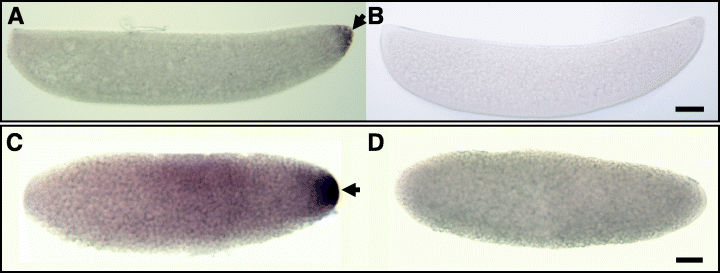
\includegraphics[width=.8\textwidth]{figures/figs/oskar_expression_AaAg.png}

\caption[\textit{oskar} gene expression in the vector mosquitoes, \Ang\ and \Aea]{\sf \textbf{\textit{oskar} gene expression in the vector mosquitoes, \Ang\ and \Aea:} \\
 Hybridizations \textit{in situ} of \textit{Anga osk} and \textit{Aeae osk} RNA probes to whole-mount \Ag\ and \Aa\ embryos. Embryos are orientated with anterior on the left. \Ag\ embryos (A,B) shown have reached cellular blastoderm with pole cells indicated by an arrow. \Aa\ embryos (C,D) shown are in the preblastoderm stage. Strong staining is exclusive to the posterior pole cells (A) and posterior end (C) (arrows), when compared with embryos of the same stage, determined by DAPI staining (not shown), probed with \textit{Anga} and \textit{Aeae osk} sense RNA probes (B,D). Bar = 50 µm.\\
 
 Excerpted from \cite{Juhn2006}}\label{fig:pole-cells}
\end{figure}

\subsection{Effector genes}

In addition to the ability to integrate transgene constructs into the vectors' genomes, it is necessary to design constructs that contain transgenes that will effect a useful response in the vector.
Two broad strategies are commonly applied when designing an anti-transmission phenotype: \gls{population-reduction} and \gls{population-conversion}.

\subsubsection{Vector population reduction:}

The goal of vector population reduction is the same as conventional vector control modalities.
\emph{Reduce the local population of a disease vector with the goal of reducing the probability that an infectious individual will have an opportunity to participate in a transmission event.}


A \textbf{transgenic tactic} for the population reduction strategy is illustrated by Oxitec's \Aa strain OX3604C developed with support from the Bill and Melinda Gates Foundation's Grand Challenges for Global Health Initiative.
Strain OX3604C represents a female-specific \gls{RIDL} approach which uses a poison transgene that kills any female adult expressing the transgene unless the female is provided an ``antidote'' through its water supply \cite{WisedeValdez2011,Bargielowski2012,Facchinelli2013}.

Releasing enough of these mosquitoes will affect the local mosquito species population in a way that is analogous to \gls{SIT}.

\subsubsection{Vector population conversion:}

Vector population conversion is a novel strategy for vector control that primarily exists within the context of genetically altered vectors (\CITEME wolbacia).
It promises to be the most long-lasting vector-focused intervention.
Unlike \textbf{all} vector population reduction tactics, there is a practical point in a conversion intervention (the anti-transmission trait works and is present in local populations at near 100\%) when the human management of the intervention can be ceased, yet it continues to function.
For population reduction to approach this result, the vector species must not simply be eliminated from the local area, but approach elimination on a continental scale, or more realistically achieve global eradication.

The reason is that these mosquitoes (especially \Aa) can and do travel long distances, as eggs or larvae, in the backs of trucks (between villages) or in the pools of water collected in super-tankers (transcontinentally).
So a local village is only free of the vectors until more migrate into the area.
But in a conversion scenario, those migrants mate with the local vector population, and their offspring are assimilated into transmission-deficient mosquitoes.
The protection of the local village can be preserved \emph{even if some surrounding villages fail to maintain control of their mosquitoes}.

An example of a \textbf{transgenic tactic} for population conversion of \Aa\ into a transmission-deficient phenotype involves an effector gene that produces a double stranded RNA molecule that contains a portion of the dengue virus genome \cite{Franz2006,Mathur2010}.
Because most animal cells have a system that detects and degrades double stranded RNA\footnote{Double stranded RNA generally signals that a virus is active in the cell.}
in a sequence specific manner, this primes the mosquito cells' antiviral response to specifically attack the dengue virus if the effector gene is expressed in the cell before it gets infected.

\subsection{Controlling when and where the effector genes are expressed}

Even with an effector gene that clears 100\% of the pathogen 100\% of the time, the intervention will not be successful in limiting transmission if the transgene is not turned on at the right time and place.
If the transgene is most effective when the pathogen is in the midgut, it is not useful if the gene is only expressed in the antennae.

The region of DNA directly before the sequence of the gene is a major determinant of the pattern of expression and is referred to as the promoter.
It influences when the gene will be turned on (e.g., directly following the ingestion of a bloodmeal), and in which tissue type (e.g., the midgut).
Promoters influence the transcription of genes through the binding of special proteins called transcription factors that recognize specific DNA sequences called \glspl{CRE}.
\glspl{CRE} are sometimes organized into modules that represent groups of binding sites for a specific combination of transcription factors.
These modules are \glspl{CRM} \CITEME (Figure \ref{fig:cre-crm-intro-a}).
Once a set of transcription factors are bound to the promoter they recruit the special machinery needed for the gene to be turned on or silenced depending on the context of the cellular environment (Figure \ref{fig:cre-crm-intro-b}).



\begin{figure}[h]

\begin{subfigure}[b]{.5\linewidth}
\centering 
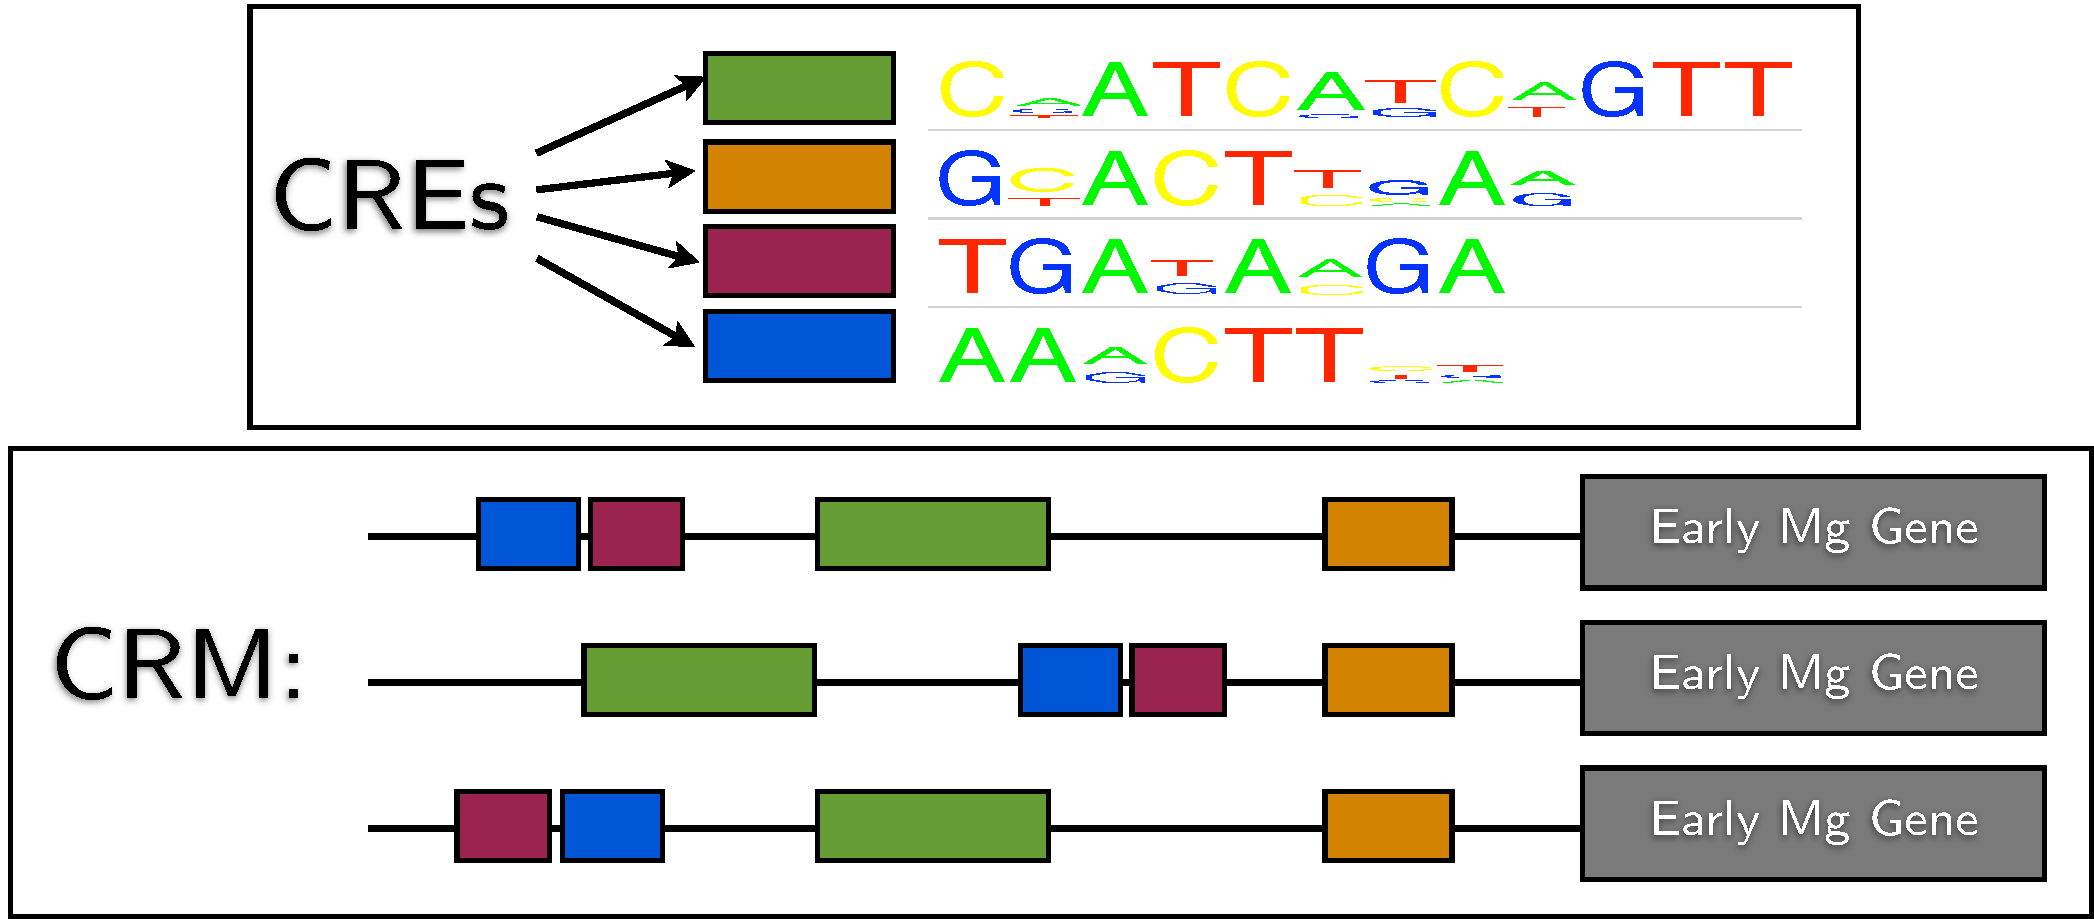
\includegraphics[width=0.9\linewidth]{figures/figs/CREvCRM.pdf}
\caption{}\label{fig:cre-crm-intro-a}
\end{subfigure}%
\hfil
\begin{subfigure}[b]{.5\linewidth}
\centering
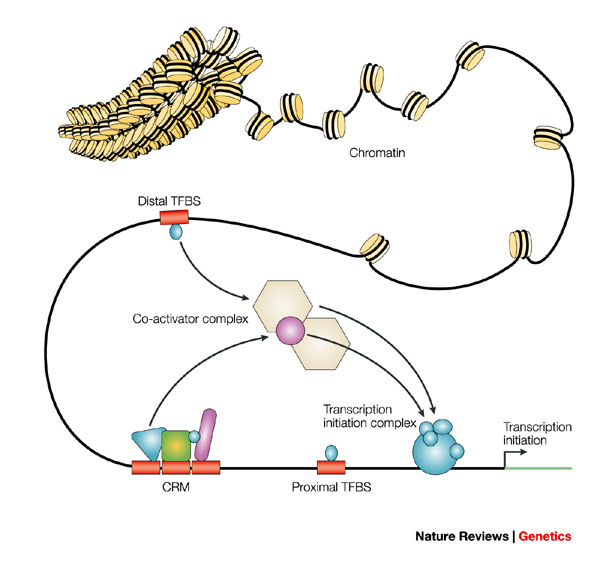
\includegraphics[width=0.9\linewidth]{figures/figs/elementsOfTxReg.jpeg}
\caption{}\label{fig:cre-crm-intro-b}
\end{subfigure}

\caption[Elements of transcriptional regulation]{\sf \textbf{Elements of transcriptional regulation} \\
(A) The relationship between \glspl{CRE} (colored rectangles) and \glspl{CRM}: the colored rectangles represent position specific scoring matrix information (top) that defines an individual \gls{CRE}.
(B) \glspl{TF} bind to specific sites (\glspl{TFBS}) that are either proximal or distal to a transcription start site. Sets of \glspl{TF} can operate in functional \glspl{CRM} to achieve specific regulatory properties. Interactions between bound \glspl{TF} and cofactors stabilize the transcription-initiation machinery to enable gene expression. The regulation that is conferred by sequence-specific binding \glspl{TF} is highly dependent on the three-dimensional structure of chromatin.\\

Panel B and corresponding legend text adapted from \citet{Wasserman2004}.
}\label{fig:cre-crm-intro}
\end{figure}

A typical strategy to obtain regulatory sequences suited to drive a transgene following the expression characteristics used as an example above (expressed directly following ,a bloodmeal, in the midgut) would be to identify genes in the mosquito that already have a similar expression pattern to the ideal.
The promoter from that gene would then be copied and inserted in front of our transgene in the final integration construct.

This is a very common process used to engineer the expression patterns of real transgenes in mosquitoes.
In \cite{Moreira2000}, the promoter sequences of a gene called carboxypeptidase (normally expressed in the midgut after a meal) from \Aa\ and \Ag\ were inserted in front of a reporter gene.

From the abstract of \cite{Moreira2000}:

\begin{quote}
Six independent transgenic lines were obtained with the AeCP construct and one with the
AgCP
construct.
Luciferase mRNA and protein were abundantly expressed in the
guts of transgenic mosquitoes in four of the six AeCP lines and in the
AgCP line.
Expression of the reporter gene was gut-specific and reached
peak levels at about 24 h post-blood ingestion.
\end{quote}

\subsection{Achieving swift, dramatic, and clinically meaningful effects on the native vector population}

In many ways, this is the most difficult part of the system.
In order for the transgene to have its self-sustaining properties as well as achieve effective anti-transmission results, it must spread through the native mosquito population to the point that the percent of individuals possessing the gene approaches 100\%.

Making the optimistic assumption that the transgene carries a negligible fitness cost
\footnote{By fitness cost/advantage here, I mean that the transgene
    causes the mosquitoes that inherit it to be either less or more
    successful at producing offspring, respectively.},
or even a slight fitness advantage, achieving near 100\% conversion could take decades.
Funding terms for efforts like this in poor nations can be closer to 5 years or less.
To enable the population conversion strategies to work, genetic ``tricks'' must be exploited that cause the gene to spread through a mosquito population \textbf{much} faster than could happen naturally.
Efforts to discover or design these \gls{gene-drive} systems are an on going and active area in this field.

An example of such a method is the Medea system successfully engineered in \Dm\ (\CITEME).

\textbf{In Brief:}
\begin{enumerate}
 \item The construct consists of a \textbf{death gene} under control of a maternal effect promoter and a \textbf{rescue gene} under control of an early embryonic promoter.
 \item The \textbf{death gene} is produced by the mother and deposited into 100\% of her developing embryos: \textit{even those that did not inherit the transgene due to mating with a wild type male.}
 \item However, since the \textbf{rescue gene} is produced by only those embryos that inherited the transgene construct, only those embryos will survive.
 \item The female has on average half as many progeny survive as usual if she mated with a wild type male, but 100\% of those that survive inherit the transgene.
 \item Over time this results in the fixation or near fixation of the transgene in the population.
\end{enumerate}


\section{Conservation of bloodmeal-regulated transcription}
\dummytext[3]

\subsection{Evolutionary relationship between mosquitoes and hematophagy}
\dummytext[3]

\subsection{Implications for design of transgenic vector control systems?}
\dummytext[3]


% \briefConclude{
% \begin{itemize}
% \item there are many but we focus on Dengue Fever and Malaria
% \item causative agents are RNA viruses and Plasmodium protists, respectively
% \item people don't give people these two diseases
% \item mosquitoes generally don't give mosquitoes these diseases
% \end{itemize}
% }
% \synopsis{
% \begin{itemize}
% \item The specifics of the transmission cycle of these diseases provides multiple targets for public health interventions
% \item focus on the human
% \item focus on the vector
% \end{itemize}
% }